\documentclass[12pt]{article}
\usepackage[hmargin={1in},vmargin={1in,1in},foot={.6in}]{geometry}   
\geometry{letterpaper}              
\usepackage{color,graphicx}
\usepackage{setspace}
\usepackage{amsmath}
\usepackage{amssymb}
\usepackage{varioref}
\usepackage{textcomp}
\usepackage{textcomp}
\usepackage{mflogo}
\usepackage{wasysym}
\usepackage[normalem]{ulem}
\usepackage{hyperref}
\usepackage{booktabs}
\usepackage{natbib}

\newcommand{\HRule}{\rule{\linewidth}{0.25mm}}

\usepackage{fancyhdr} % This should be set AFTER setting up the page geometry
\pagestyle{plain} % options: empty , plain , fancy
\lhead{}\chead{}\rhead{}
\renewcommand{\headrulewidth}{.5pt}
\lfoot{}\cfoot{\thepage}\rfoot{}
\newcommand{\txtp}{\textipa}
\renewcommand{\rm}{\textrm}
\newcommand{\sem}[1]{\mbox{$[\![$#1$]\!]$}}
\newcommand{\lam}{$\lambda$}
\newcommand{\lan}{$\langle$}
\newcommand{\ran}{$\rangle$}
\newcommand{\type}[1]{\ensuremath{\left \langle #1 \right \rangle }}

\newcommand{\bex}{\begin{exe}}
\newcommand{\eex}{\end{exe}}
\newcommand{\bit}{\begin{itemize}}
\newcommand{\eit}{\end{itemize}}
\newcommand{\ben}{\begin{enumerate}}
\newcommand{\een}{\end{enumerate}}

\newcommand{\gcs}[1]{\textcolor{blue}{[gcs: #1]}}

\thispagestyle{plain}

\title{Subjectivity predicts adjective ordering preferences}
\author{Gregory Scontras, Judith Degen, Noah D.~Goodman}
%\date{}

\begin{document}

\maketitle

Regularities in the behavior of speakers and speech communities provide a window onto the psychology of language. Here we take up one such regularity: adjective ordering. Speakers and listeners exhibit strong ordering preferences when two or more adjectives are used to modify a noun, as in ``the big blue box'' or ``the good smooth purple plastic chair.'' Deviate from the preferred order, and the construction becomes odd. Something feels particularly unwieldy about ``the blue big box,'' even more so with ``the plastic good purple smooth chair.'' 
Why do most strings of adjectives have tightly-constrained order? 
We investigate the role of adjective meaning, specifically the subjectivity of the properties that the adjectives name, in predicting ordering preferences.

Adjective ordering preferences stand as a particularly striking case of regularity in language. More remarkable than their robustness in English is their cross-linguistic systematicity: we continually find the \emph{same} preferences across the world's languages. Hungarian (Uralic), Telugu (Dravidian), Mandarin Chinese, and Dutch are just a handful of languages with pre-nominal adjectives (i.e., languages where adjectives precede nouns) reported to have the same ordering preferences as English \citep{Martin1969a,hetzron1978,dixon1982,Sproat1991,LaPolla2004}.  In languages like Selepet (Papuan) and Mokilese (Micronesian) with post-nominal adjectives (i.e., where adjectives follow nouns), these preferences are preserved in the reverse \citep{hetzron1978,dixon1982,Sproat1991}---stable preferences determine the linear distance of an adjective from the noun it modifies.

There have been two general approaches to the investigation of adjective ordering preferences. 
As part of a larger project mapping the syntax and semantics of adjectives (a ``cartographic'' approach, one could say), the linguistics literature advances a universal hierarchy of semantic classes of adjectives. Leading the charge, \citet{dixon1982} set out to uncover language-internal structure by which to organize ordering preferences. The preferences were assumed to be hard-coded in the grammar; the researcher's job was simply to uncover them. 
Building on the ordering of semantic classes proposed by Dixon, \cite{Cinque1994} advanced a fully syntactic account of ordering preferences under which different classes of adjectives populate dedicated syntactic categories which inhabit specialized projections in the syntactic tree. For example, color adjectives project a Color Phrase, shape adjectives project a Shape Phrase. The Shape Phrase syntactically dominates the Color Phrase; with left-branching structure, hierarchical dominance results in linear precedence. The ultimate source of this rigid structure was immaterial; at issue was a comprehensive and deterministic account of the facts (see \citealp{scott2002} for a similar proposal). 

Before the grammatical approaches, which map, as it were, the terrain of adjective \emph{structure}, psychological approaches advanced the idea that aspects of adjectives' \emph{meaning} determine their relative order. The trouble lies in deciding precisely which aspects of meaning are relevant. 
Kicking off the enterprise in \citeyear{sweet1898}, \citeauthor{sweet1898} proposed that adjectives which are more closely connected with the noun in meaning occur closer to the noun, and that adjectives with a more specialized meaning occur closer to the noun. Similarly, \cite{whorf1945} proposed that adjectives describing more ``inherent'' properties occur closer to the noun. \cite{ziff1960} proposed that adjectives with less context-dependent meaning occur closer to the noun, and that adjectives that felicitously describe a narrower set of nouns occur closer to the noun. Recent compositional approaches have argued that the fundamental factor in predicting adjective ordering is whether or not an adjective forms a new concept with the noun it modifies \citep{McNally2004,svenonius2008}: first you form the concepts (e.g., ``wild rice'' or ``bad apple''), then you modify them (e.g, ``Minnesotan wild rice'').  These proposals and others like them circle around similar aspects of adjective meaning in their account of ordering preferences; unfortunately, operationalizing metrics like meaning distance, specificity, inherence, and context-dependence is not a trivial task (but see the attempt in \citealp{martin1969}). 
Lacking clear empirical measures of the relevant aspects of adjective meaning, these psychological accounts gave way to the more descriptive, grammatical ones that settle for innate syntax as the ultimate arbiter. 

We revisit the idea that ordering preferences emerge from aspects of adjective meaning, attempting to provide more thorough empirical grounding to these notions;
from the grammatical approach we adopt the strategy of using semantic classes of adjectives to structure our investigation and smooth our data. 
Distilling the psychological proposals that precede us into a single feature, we advance the hypothesis that it is the \emph{subjectivity} of the property named that determines ordering preferences \citep{hetzron1978,Quirk1985,hill2012}.
Less subjective adjectives are reliably more useful at communicating the speaker's intended message; the chance of miscommunication decreases with decreasing subjectivity. 
Perhaps for this reason, less subjective adjectives occur closer to the substantive head of the nominal projection, that is, to the modified noun?  
%We show that adjective subjectivity can be assessed directly (by asking participants); we validate this measure  as the extent to which two people can disagree about a description without one necessarily being wrong. 
In ``the big blue box,'' judgments about bigness are likely less consistent than judgments about blueness; ``blue'' is less subjective than ``big,'' and so, according to this theory, it occurs closer to the noun ``box.''

To test the hypothesis that adjective subjectivity predicts ordering preferences, we created and validated empirical measures of the ordering preferences themselves and of an adjective's subjectivity. With reliable estimates of both, we then evaluated the predictive power of subjectivity in adjective ordering preferences. Next, we investigated the role of specific noun information in the determination of ordering preferences. Finally, we extended our empirical coverage to a larger set of adjectives and nouns.

\section{Experiment 1: Establishing the measures}

\subsection{Ordering preferences}

We began by measuring preferences in adjective ordering. We selected a sample of 26 relatively frequent, imageable adjectives from seven different semantic classes discussed in the grammatical literature (dimension, value, age, physical, shape, color, material). 
%"age","color","dimension","human","location","material","nationality","physical","shape","speed","temporal","value"
We then elicited naturalness judgments on adjective-adjective-noun object descriptions, permuting the relative order of the adjectives.

\begin{table}[t]
	\caption{Adjectives and their semantic classes tested in all experiments, and nouns and their classes tested in the behavioral experiments.}\label{stim-table}
	\centering{\footnotesize\begin{tabular}{@{\vrule height 10.5pt depth2pt  width0pt}llll|ll}\\
	\toprule
			Adjective	&	Class	&	Adjective	&	Class	&	Noun	&	Class	\\ \midrule
			old	&	age	&	good	&	value	&	apple	&	food	\\
			new	&	age	&	bad	&	value	&	banana	&	food	\\
			rotten	&	age	&	round	&	shape	&	carrot	&	food	\\
			fresh	&	age	&	square	&	shape	&	cheese	&	food	\\
			red	&	color	&	big	&	dimension	&	tomato	&	food	\\
			yellow	&	color	&	small	&	dimension	&	chair	&	furniture	\\
			green	&	color	&	huge	&	dimension	&	couch	&	furniture	\\
			blue	&	color	&	tiny	&	dimension	&	fan	&	furniture	\\
			purple	&	color	&	short	&	dimension	&	TV	&	furniture	\\
			brown	&	color	&	long	&	dimension	&	desk	&	furniture	\\
			wooden	&	material	&	smooth	&	physical	\\				
			plastic	&	material	&	hard	&	physical	\\				
			metal	&	material	&	soft	&	physical	\\	\bottomrule												
		\end{tabular}} 
\end{table}


\paragraph{Participants.} We recruited 50 participants through Amazon.com's Mechanical Turk crowd-sourcing service. Participants were paid \$0.30 for their participation. 

\paragraph{Design and methods.} Participants were asked to indicate which of two descriptions of an object sounded more natural. Each description featured a noun modified by two adjectives, for example ``the red small chair'' or ``the small red chair''. Descriptions were random combinations of two adjectives and a noun from the list in Table \ref{stim-table}, with the constraint that no description contained adjectives from the same semantic class. Description pairs contained the same words, with relative adjective order reversed. 
On each trial, participants indicated their choice by adjusting a slider with endpoints labeled with the competing descriptions; an example trial appears in Fig.\ \ref{order-trial}. Participants completed 26 trials. On each trial, we measured the distance of the slider from each endpoint; values ranged between 0 and 1. Only native speakers of English with IP addresses located within the United States were included in the analyses; we analyzed data from 45 participants. 

\begin{figure}[h]
	\centering
	\fbox{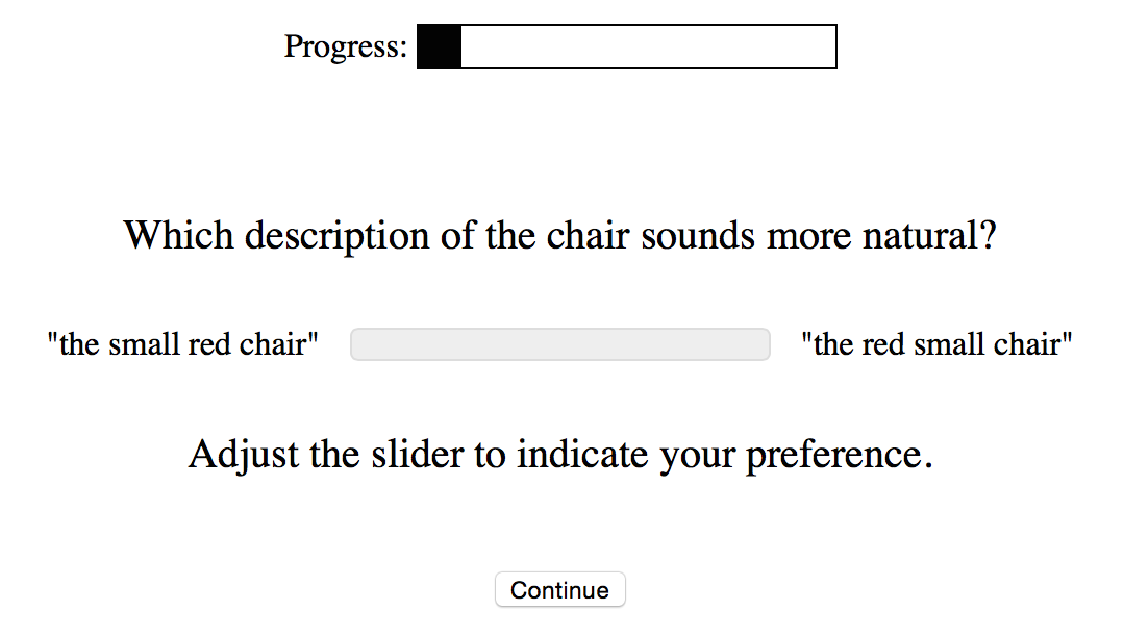
\includegraphics[width=3.3in]{images/order_trial.eps}}
	\caption{Example trial from \emph{Expt.\ 1.1 Ordering preferences}; participants indicated the more natural of two adjective-adjective-noun descriptions on a sliding scale.}\label{order-trial}
\end{figure}

\begin{figure}[tbh]
	\centering
	{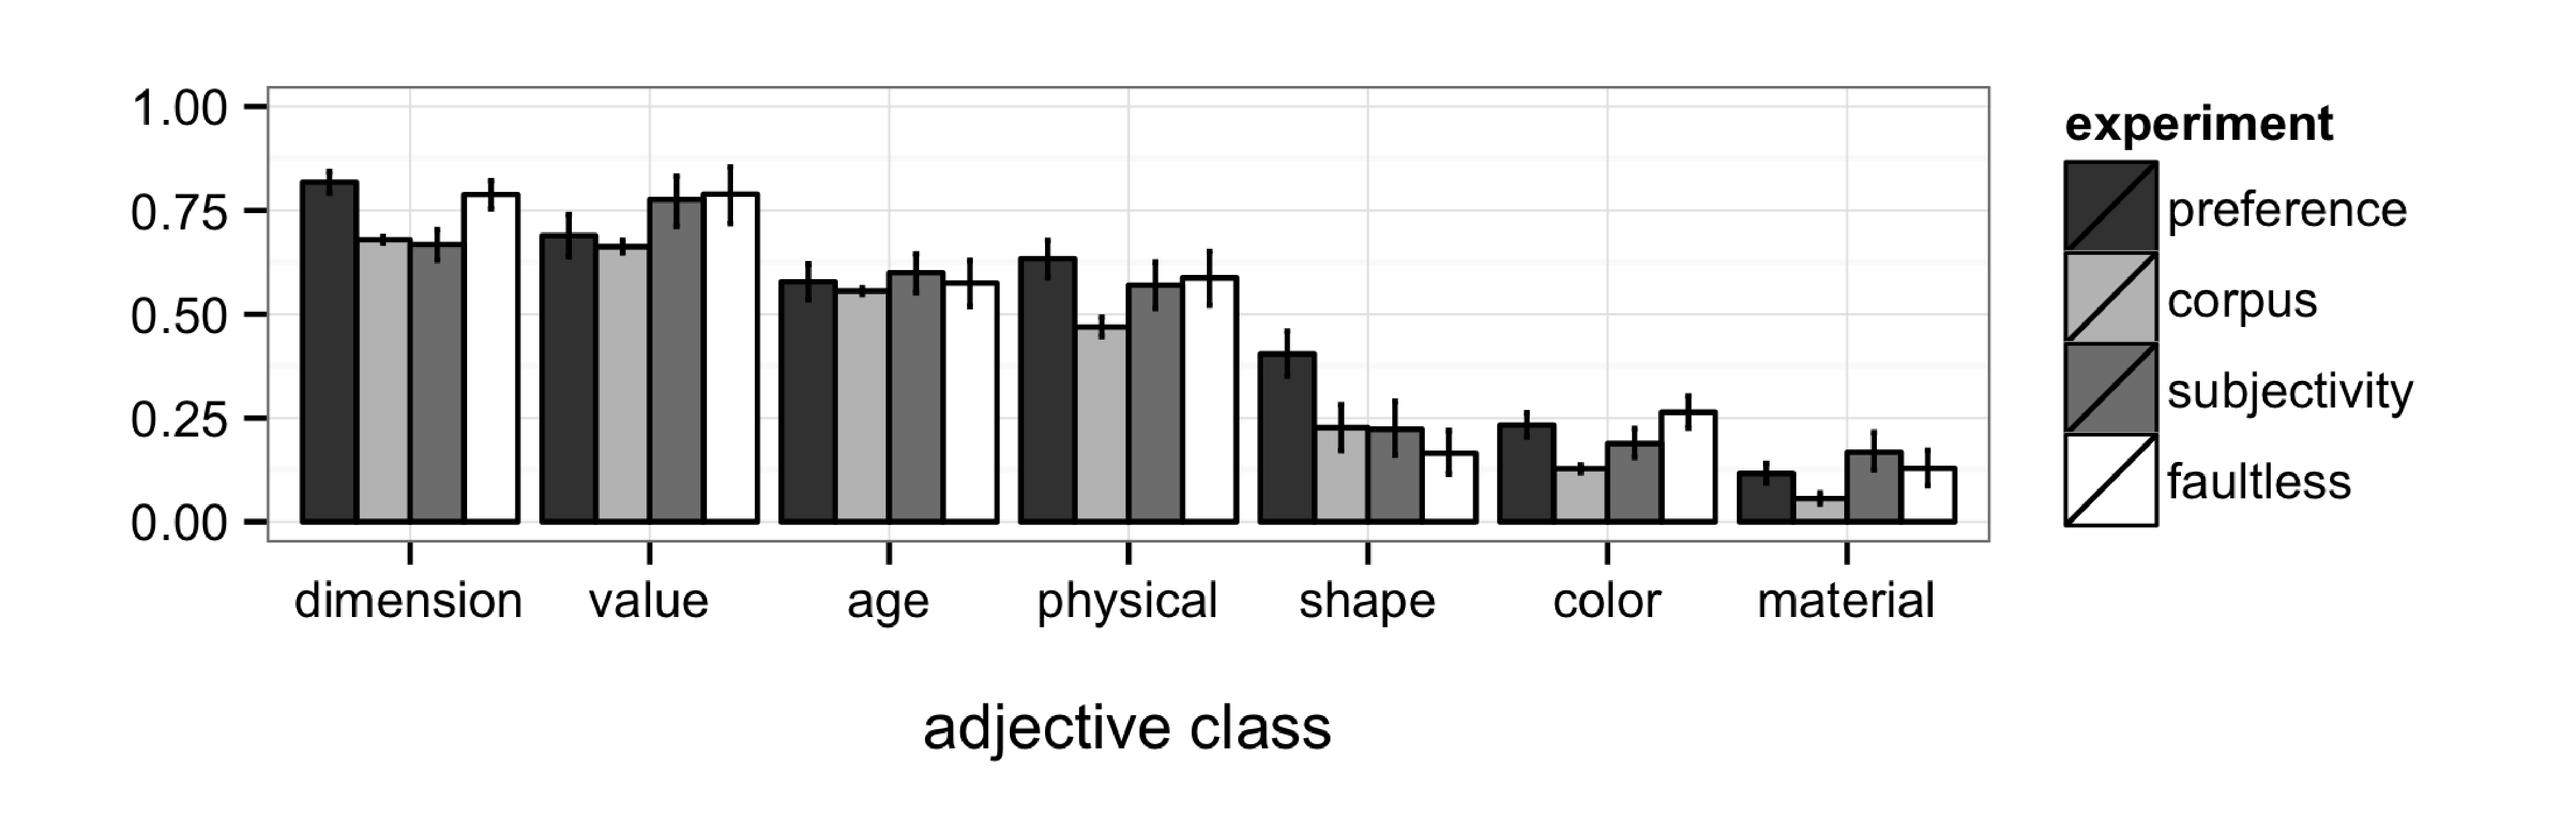
\includegraphics[width=.75\linewidth]{plots/expt_results-new.eps}}\par
	\caption{Mean distance from noun inferred from naturalness ratings (\emph{preference}), mean distance from noun calculated from corpus counts (\emph{corpus}), mean subjectivity ratings (\emph{subjectivity}), and mean faultless disagreement ratings (\emph{faultless}) for adjectives grouped by their semantic class. Error bars represent bootstrapped 95\% confidence intervals drawn from 10,000 samples of the data \citep{DiCiccio1996}.}\label{results}
\end{figure}

\paragraph{Results.} For each adjective, we computed its mean naturalness score by averaging ratings of configurations in which it appeared in first position, farthest from the noun. Fig.\ \ref{results} (\emph{naturalness}) plots these mean naturalness scores by adjective class; greater values signal that a class's adjectives are preferred in first position, while lower values indicate that a class's adjectives are preferred in second position, closer to the noun. This preferred distance measure closely tracks class-level ordering hierarchies reported in the literature \citep{dixon1982,Sproat1991}.

\paragraph{Corpus validation.} To validate our behavioral measure of ordering preferences, we conducted a corpus study on the same 26 adjectives and measured their mean distance from the noun in phrases with two adjectives. We used TGrep2 \citep{rohde2005} and the TGrep2 Database Tools \citep{Degen2011} to extract all ``A A N"  NPs that contained one of the 26 adjectives in Table \ref{stim-table} from the Penn Treebank subset of the Switchboard corpus of telephone dialogues \citep{godfrey1992}, as well as from the spoken and the written portions of the British National Corpus (BNC, see http://www.natcorp.ox.ac.uk/). For these cases, we computed the distance of each occurrence of our 26 target adjectives from the modified noun, yielding results for a total of 38,418 adjective tokens.  For each adjective, mean distance from the noun was computed (where the position directly preceding the noun was coded as 0, and the position preceding that was coded as 1). The procedure described above was used to compute mean distance by adjective class.

Mean distance from the noun for each adjective class is shown in Fig.~\ref{results} (\emph{corpus}); higher values indicate that adjectives from the specified class tend to appear farther from the modified noun. The corpus measure closely tracks the qualitative pattern we measured in our naturalness experiment; quantitatively, the two measures are highly correlated ($r^{2}=0.83$, 95\% CI [0.63, 0.90]), in spite of the fact that the corpus measure includes cases from a superset of the nouns tested in our naturalness experiment. Our naturalness ratings thus operationalize both immediate ordering preferences and speakers' preferences in natural usage.

\paragraph{Looking for noun effects.} We next asked to what extent ordering preferences depend on the modified noun. Analyses of adjective semantics hold that adjectives that form idiomatic concepts or natural kinds (e.g., ``bad apple'' or ``blue cheese'') compose first with nouns, before run-of-the-mill intersective adjectives, thus enforcing a strict ordering \citep{McNally2004,svenonius2008}; we might therefore expect to find that adjectives that compose with a noun to yield an idiomatic concept are preferred linearly closer to the modified noun. 
To evaluate the role of specific noun information in determining ordering preferences, we performed a nested linear model comparison. The models predicted naturalness ratings either by \textsc{adjective} (i.e., the adjective farthest from the noun) only, or by \textsc{adjective} together with its interaction with \textsc{noun} (i.e., the modified noun).
The model comparison revealed that noun-specific ratings did not explain any additional variance in ordering preference above and beyond adjective-level ratings ($F(1,234) = 1.10, p < 0.15$).  Thus, we fail to find evidence of noun-specific effects on ordering preferences in our materials. However, there remains the possibility that our materials (i.e., nouns and adjectives) did not yield sufficiently idiomatic object descriptions that would deliver these noun-specific effects. We follow up on this possibility in Experiment 2.


\subsection{Subjectivity}

With clear estimates of ordering preferences, we then measured the subjectivity of the adjectives that were tested in the ordering preferences experiment. We started with a direct measure: participants were asked explicitly to rate the ``subjectivity'' of our adjectives.

\paragraph{Participants.} We recruited 30 participants through Amazon.com's Mechanical Turk crowd-sourcing service. Participants were paid \$0.30 for their participation. 

\paragraph{Design and methods.} Participants were shown a series of adjectives and asked to indicate how ``subjective'' each one was on a sliding scale with endpoints labeled as ``completely objective'' (coded as 0) and ``completely subjective'' (coded as 1; Fig.~\ref{subjectivity-trial}). 
%Adjectives were chosen at random from the list in Table \ref{stim-table}. 
Participants completed a total of 26 trials, one for each adjective in Table \ref{stim-table}. The order was randomized for each participant. Only native English speakers with IP addresses located within the United States were included in the analyses; we analyzed data from 28 participants.

\begin{figure}[tbh]
	\centering
	\fbox{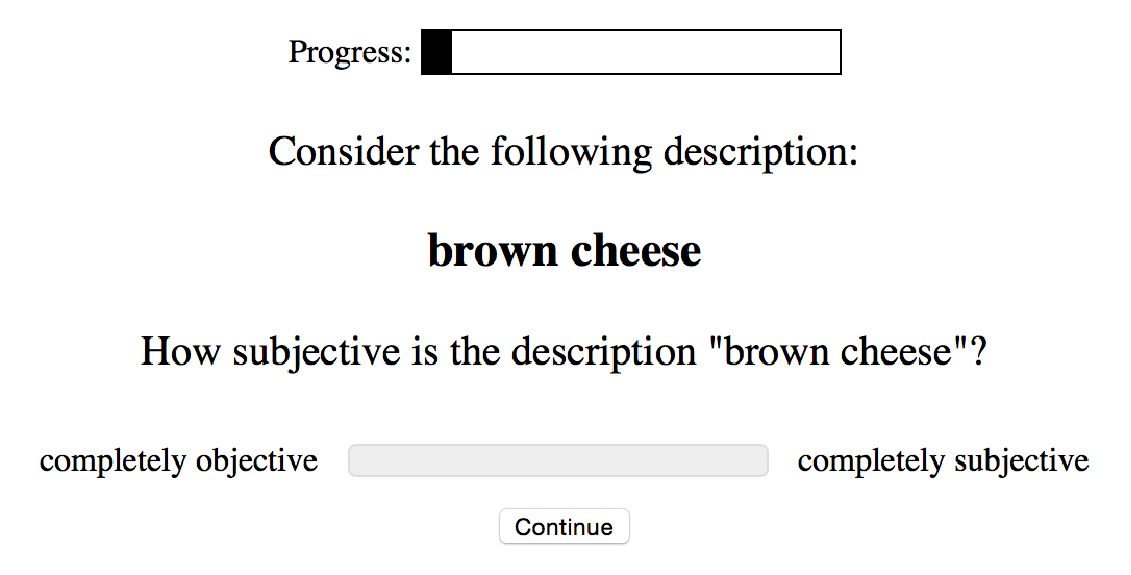
\includegraphics[width=3.3in]{images/subjectivity_trial.eps}}
	\caption{Example trial from \emph{Expt.\ 1.2 Subjectivity}; participants rated the subjectivity of adjectives.}\label{subjectivity-trial}
\end{figure}

\paragraph{Results.} We averaged the subjectivity scores for each adjective; greater values indicate greater subjectivity. These averages were used in the analyses reported below. Fig.\ \ref{results} (\emph{subjectivity}) show these scores by adjective class.

\paragraph{Faultless disagreement validation.} Because subjectivity may be an ambiguous, or even subjective, property, we explored a second measure that may have greater ecological validity. 
We operationalized subjectivity as the potential for faultless disagreement between two speakers, which captures potential uncertainty about assessment criteria and assessment outcomes \citep{Kolbel2004,kennedy2013,barker2013}.\footnote{See \cite{MacFarlane2014} for more discussion of the many factors, both ``semantic'' and ``pragmatic,'' that contribute to faultless disagreement effects. For a different approach, see \cite{hill2012}, who builds on previous corpus work \citep{wulff2003} to infer adjective subjectivity from surface features of strings.}
We had participants (n=40) evaluate whether two speakers could both be right while the speakers produced conflicting object descriptions. For example, an experimental trial would have Mary assert, ``That apple is old,'' then have Bob counter with ``That apple is not old;'' 
participants rated whether both Mary and Bob could be right, or whether one of them must be wrong. This measure, the faultless disagreement potential for the adjective at issue, serves as an empirical estimate of adjective subjectivity. 
Fig.\ \ref{results} (\emph{faultless}) plots these scores by adjective class, where a value of 1 signals that a class's adjectives are always amenable to faultless disagreement (i.e., maximally subjective), and a value of 0 indicates that a class's adjectives are never amenable to faultless disagreement (i.e., minimally subjective).
The results of this method were highly correlated with our direct ``subjectivity'' scores ($r^{2} = 0.91$, 95\% CI [0.86, 0.94]), suggesting that they measure a common underlying value---adjective subjectivity. 

%\gcs{faultless disagreement methods} We recruited 40 participants through Amazon.com's Mechanical Turk crowd-sourcing service. Participants were paid \$0.35 for their participation. Participants saw a series of short dialogues in which speakers disagreed about an object that they both could see.  Their task was to determine ``whether one speaker must be wrong, or whether both speakers can be right'' using a sliding scale with endpoints labeled ``No, somebody must be wrong'' (coded as 0)  and ``Yes, it's a matter of opinion'' (coded as 1). Speaker names were chosen at random. The object name was randomly chosen from the set of nouns in Table \ref{stim-table}, and the predicate was randomly chosen from the set of adjectives. Whether the initial statement was positive or negative was chosen at random for each trial. In the example trial in Fig.~\ref{faultless-trial}, the initial statement is negative, the predicate is ``tiny,'' and the noun is ``couch.'' Participants completed a total of 26 trials, one for each of the adjectives in Table \ref{stim-table}.
%All 40 participants were native speakers of English with IP addresses located within the United States, so we analyzed data from all 40 participants.

\subsection{Predicting adjective order}

To evaluate the power of subjectivity in predicting adjective ordering preferences, Fig.~\ref{naturalness-subjectivity-pred} plots mean naturalness ratings (Expt.~1.1) against mean adjective subjectivity scores (Expt.~1.2). Adjective subjectivity scores account for  85\% of the variance in the naturalness ratings ($r^2$ = 0.85, 95\% CI [0.75, 0.90]).
The faultless disagreement scores also perform well, accounting for 88\% of the variance ($r^2$ = 0.88, 95\% CI [0.77, 0.95]).  
Using either measure, more subjective adjectives are preferred farther from the noun; subjectivity indeed predicts adjective ordering preferences.

\begin{figure}
	\centering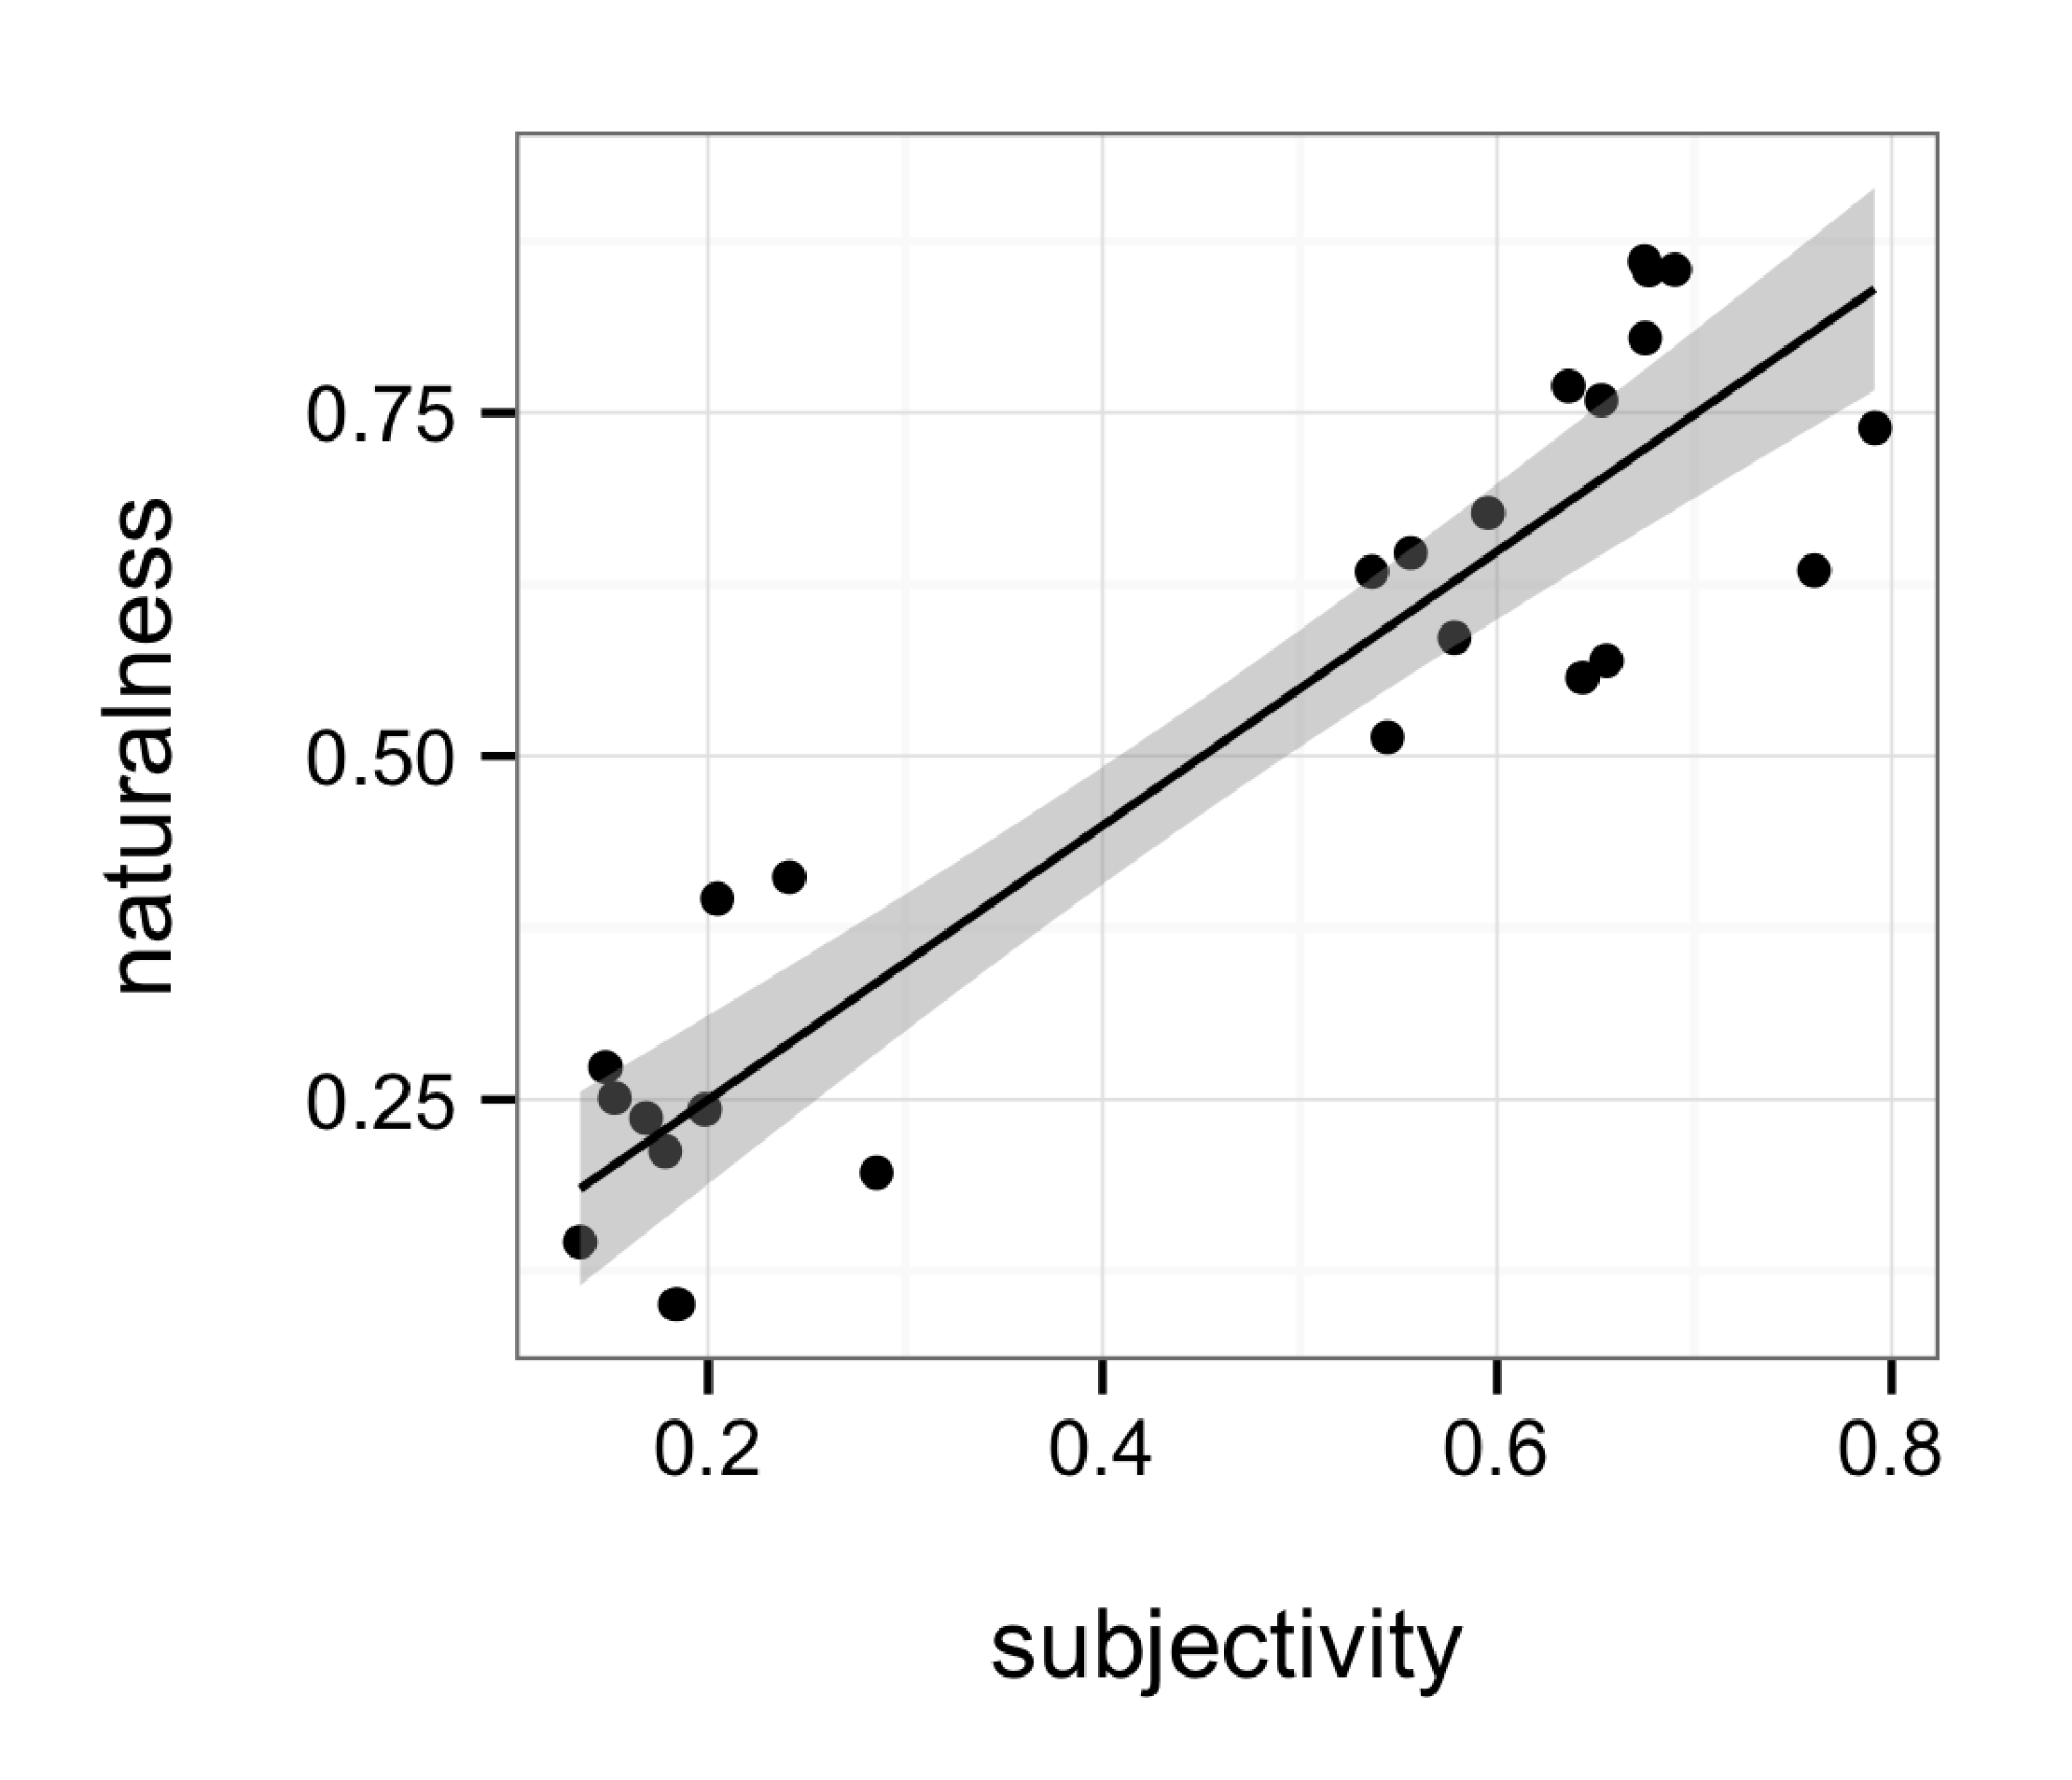
\includegraphics[width=3.5in]{plots/naturalness-subjectivity-new.eps}
	\caption{Mean naturalness ratings plotted against mean subjectivity scores for each of the 26 adjectives tested in Expt.~1.}\label{naturalness-subjectivity-pred}
\end{figure}

One might worry that conducting our analysis at the level of individual adjectives obscures information about the specific adjective-adjective configurations that participants rated in our naturalness experiment.
We therefore computed a subjectivity difference score for each adjective class configuration (i.e., an ordered pairing of two adjective classes, \textsc{class1}-\textsc{class2}) by subtracting the mean subjectivity score for \textsc{class2} from the mean subjectivity score for \textsc{class1}. Higher difference scores indicate that the adjective class closer to the noun is less subjective than the class farther away. Fig.~\ref{naturalness-subjectivity} plots mean naturalness ratings for adjective class configurations against these subjectivity difference scores; the two measures are highly correlated ($r^2$ = 0.80, 95\% CI [0.68, 0.88]).\footnote{If we analyze faultless disagreement difference scores instead, we find that they also account for significant variance in the configuration naturalness ratings ($r^2$ = 0.82, 95\% CI [0.71, 0.88]).}

\begin{figure}
	\centering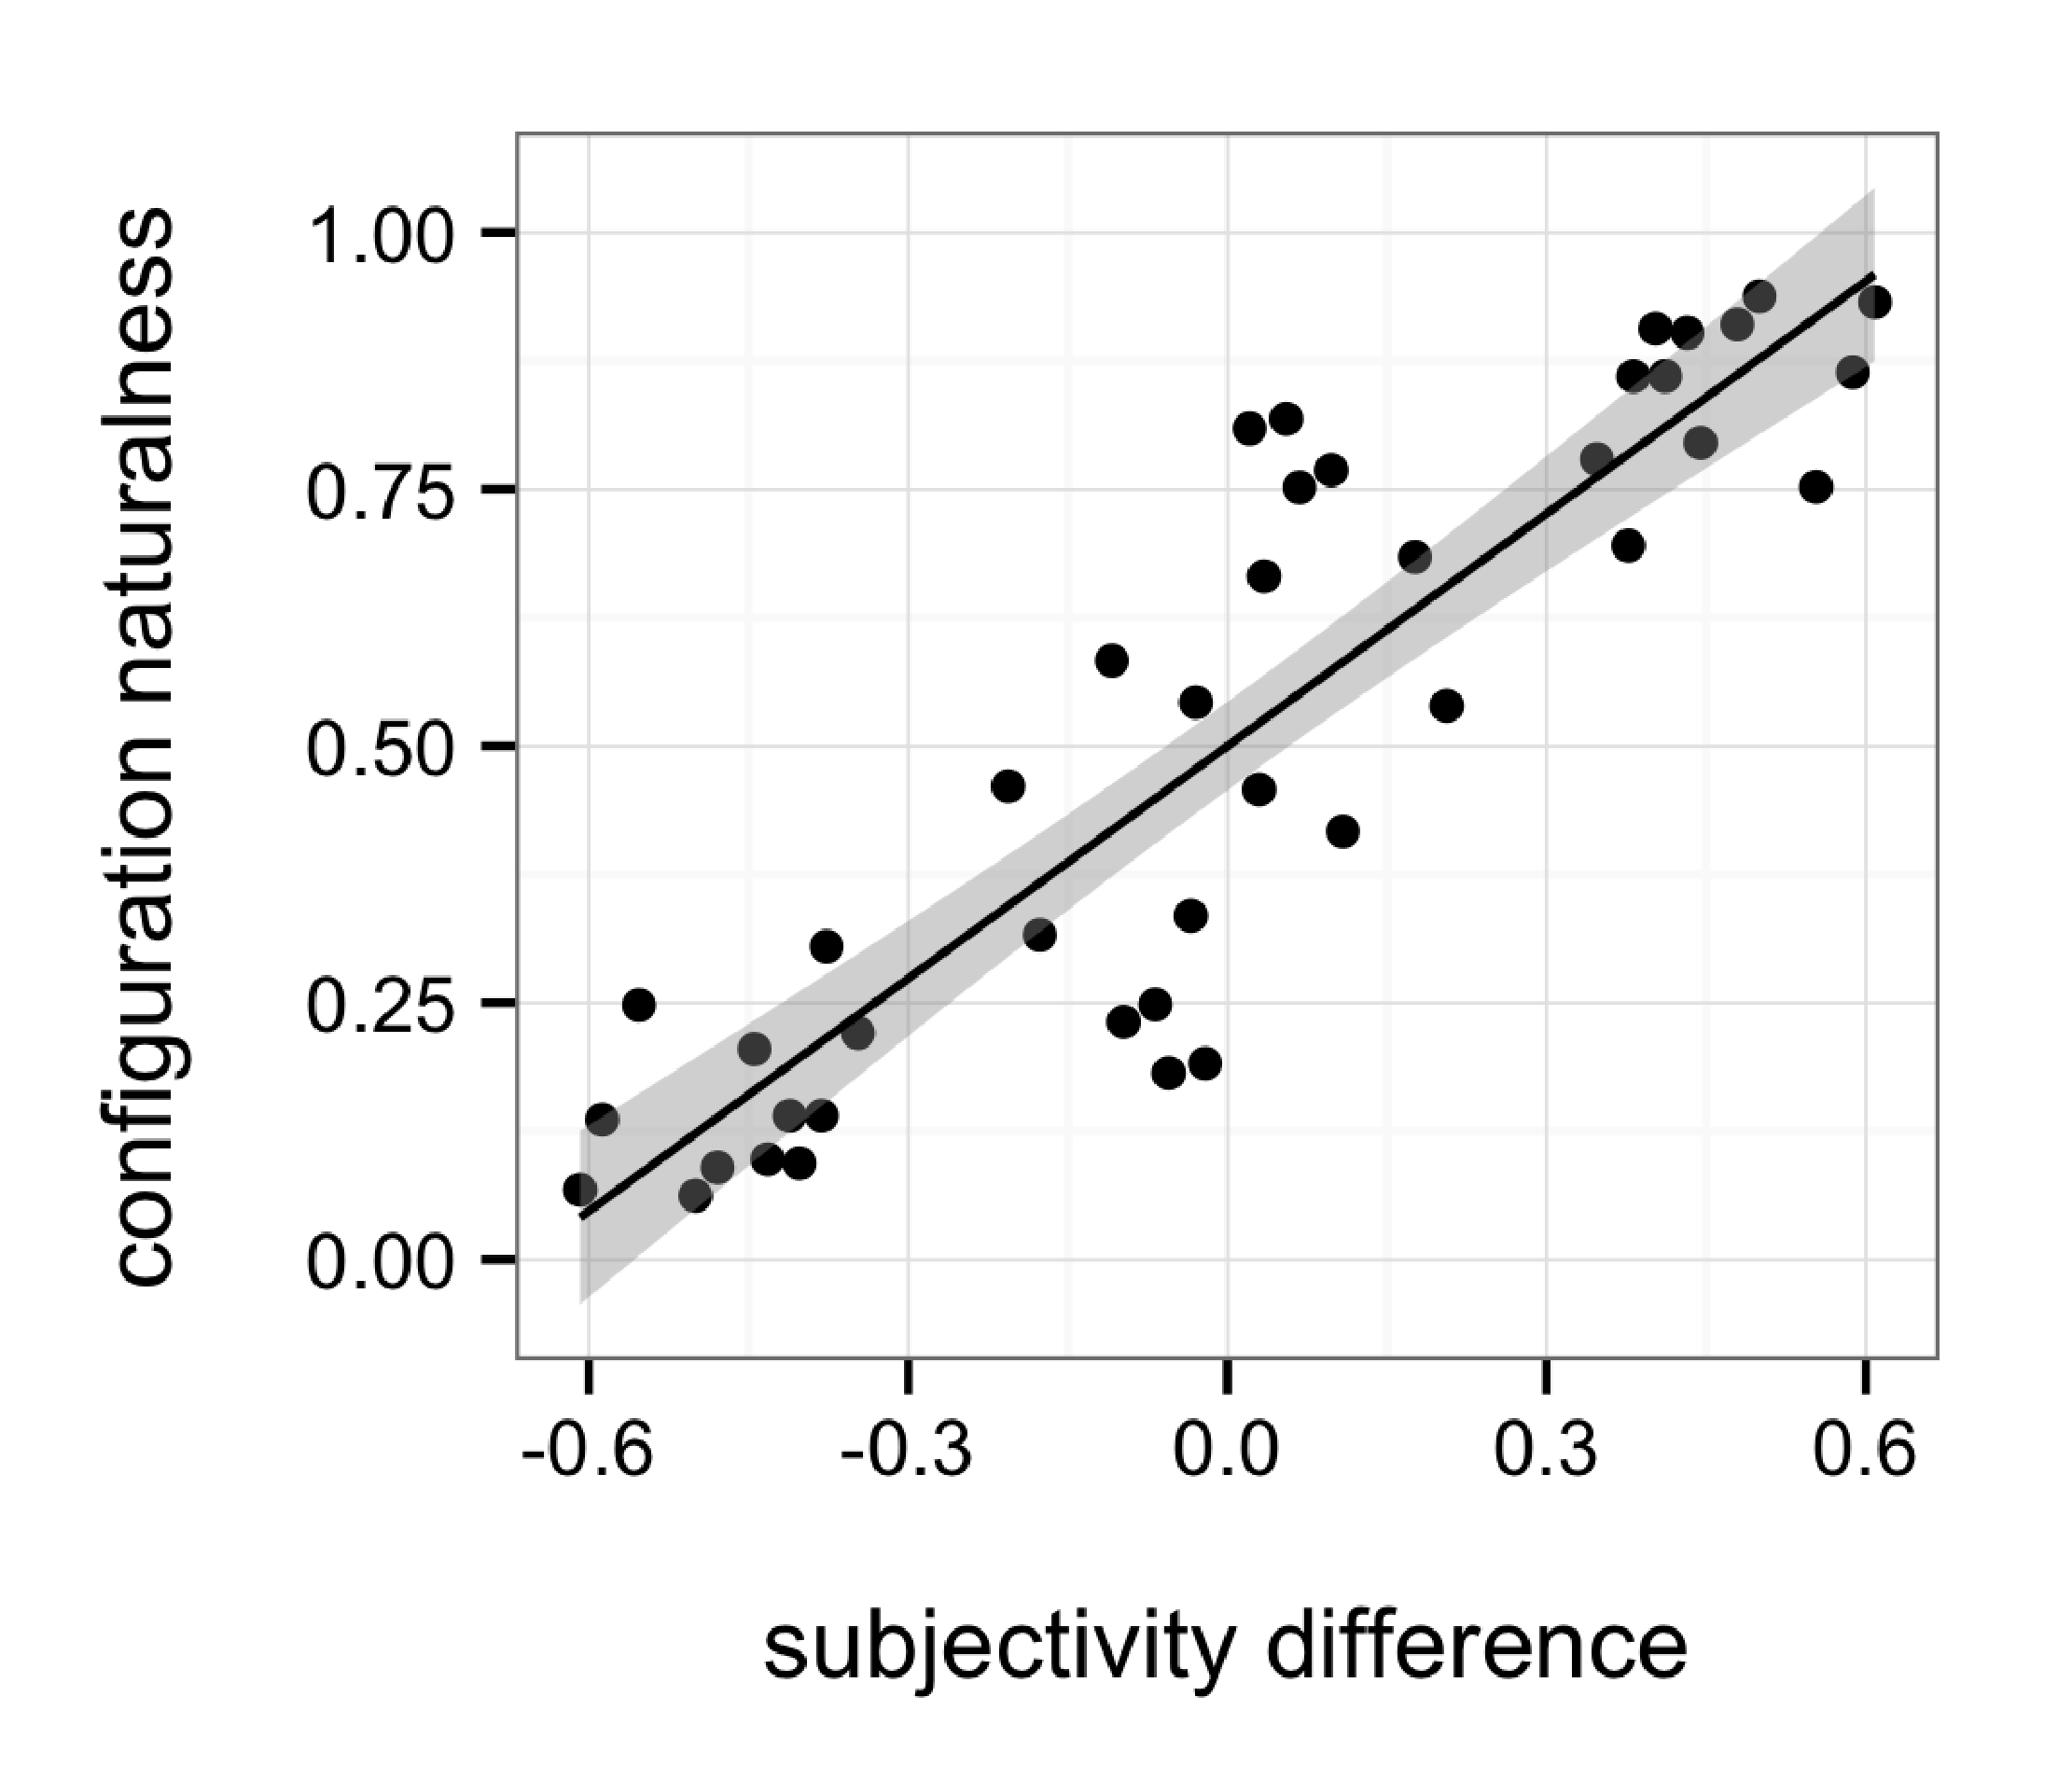
\includegraphics[width=3.5in]{plots/naturalness-subjectivity-configuration.eps}
	\caption{Mean configuration naturalness ratings plotted against subjectivity difference scores for each pair of adjective classes tested in Expt.~1.}\label{naturalness-subjectivity}
\end{figure}

%Performing the same analysis on specific adjective configurations, we find that subjectivity difference scores predict 66\% of the variance in the rating data ($r^2$ = 0.66, 95\% CI [0.61, 0.70]), which constitutes 80\% of the theoretical maximum (i.e., variance not due to noise). To compute the explainable variance in the naturalness rating data, we first computed the split-half correlation of the data to itself. To do so, we chose a random sample of 23 participants, then correlated their data with the data from the remaining 22 participants. We repeated this process 100 times; the mean split-half correlation of our data was 0.70. To ``step up'' the split-half correlation to provide an estimated correlation of the data with itself, we entered this value into the Spearman-Brown Prophecy formula \citep{stanley1971}. The result, 0.82, signals that 82\% of the rating data is explainable, that is, not due to noise.

\subsection{Discussion}

We found that adjective subjectivity scores account for a great deal of the variance in naturalness ratings, for several different analyses, strongly supporting our hypothesis that less subjective adjectives occur closer to the noun. We generalize this finding to a broader set of adjectives in Expt.~3, but first we explore in more detail whether the modified noun affects ordering preferences of the adjectives that modify it.

%However, we were surprised to learn that noun-specific information did not affect ordering preferences in our materials. Could it be that ordering preferences are independent of the modified noun? We more directly address this question in Expt.~2 with a new set of nouns.

%A more theoretically neutral version of this hypothesis is that some interaction between the noun and adjective will determine how closely the adjective is placed to the noun. This interaction could be caused by concept-formation, differential subjectivity, or other factors. 
%In Expt.~2, we follow up on this result by replicating our naturalness rating experiment with a new set of nouns chosen to maximize the probability of by-noun effects.

%Compound concepts will be described using the two-word name, presumably yielding more occurrences of this bigram than would be expected from the unigram frequencies of the noun and adjective. We thus chose new nouns whose co-occurrence probability with our 26 adjectives in the BNC is far greater than one would predict on the basis of their individual word probabilities: \emph{apple, cheese, eyes, hair}. We also included the noun \emph{thing} because it occurred naturalistically with the greatest number (23) of our 26 adjectives.

%
%\begin{figure}[h]
%	\centering
%	\fbox{\includegraphics[width=3.75in]{images/faultless_trial.eps}}
%	\caption{Example trial from Expt.\ 3; participants rated the potential for faultless disagreement between two speakers.}\label{faultless-trial}
%\end{figure}










\section{Experiment 2: In search of noun effects}

Compositional accounts of ordering preferences hold that the fundamental factor in predicting adjective ordering is whether or not an adjective is used to form a complex concept/subkind description: first you form the concept, then you modify it with additional adjectives \citep{McNally2004,svenonius2008}.\footnote{\cite{bouchard2005} makes a similar claim, namely that the formation of complex concepts can override adjective ordering preferences.} 
This would imply that an interaction between the noun and a modifying adjective---whether they combine to form a complex concept---should have a large influence on adjective ordering. 
Indeed, a more general hypothesis is that \emph{some} interaction between a noun and adjective will influence how closely the adjective is placed to that noun. This interaction could be caused by concept-formation, differential subjectivity, or other factors. We tested for such an interaction in Expt.~1 and found that noun-specific naturalness did not explain any variance in ordering preference above and beyond adjective-level naturalness. Looking in more detail, there were two adjective-noun pairs in our data with trends in the predicted direction: the naturalness ratings for \emph{hard} and \emph{soft} suggested a preference to occur closer to the noun \emph{cheese}. (Plausibly because hard and soft cheeses are natural kinds.) While these adjective-noun interactions do not survive correction for multiple comparisons in our statistical analysis, they do indicate that a different set of materials might reveal by-noun effects on ordering preference. Here we follow up on this result with a new set of materials that were chosen to maximize the probability of noun effects.


\subsection{Ordering preferences}

This experiment was a direct replication of \emph{Expt.~1.1 Ordering preferences}, using a different set of nouns. We aimed to choose nouns that formed idiomatic, complex concepts with our previous set of adjectives. Complex concepts tend to be described using the two-word name, yielding more occurrences of this bigram than would be expected from the unigram frequencies of the noun and adjective. This provided a way to extract candidate complex concepts from corpora.

 %with the given adjectives and therefore yield effects on ordering preferences.

\paragraph{Participants.}

We recruited 50 participants through Amazon.com's Mechanical Turk crowd-sourcing service. Participants were compensated for their participation.

\paragraph{Design and methods.}

The design was identical to our original naturalness ratings experiment: participants were asked to indicate which of two object descriptions sounded more natural, using a sliding scale. Each description featured a noun modified by two adjectives; description pairs contained the same words with the relative adjective order reversed (e.g., ``the big blue thing'' vs.~``the blue big thing''). Adjectives were chosen at random from the original set of 26. The nouns were a smaller set of five (compared to the original ten). Nouns were chosen to maximize the probability of detecting noun-specific effects on adjective ordering preferences. In particular, we expected that nouns that are likely to form complex concepts should be 
highly collocational with that adjective. We thus searched for nouns that occur in particular adjective-noun phrases more frequently than predicted by the individual noun and adjective probabilities; in other words, nouns whose adjective-noun combinations were under-predicted by their individual word probabilities. 

To find these nouns, we estimated the probability $p(A)$ of each adjective from our set of 26 by computing its relative frequency in an adjective-noun sequence in the BNC. We then computed the relative frequency of each noun $p(N)$ occurring in an adjective-noun sequence. Finally, we estimated the predicted joint probability of each adjective-noun combination by taking the product of each individual probability estimate: $\hat{p}(A,N) = p(A)\cdot p(N)$. Comparing  $\hat{p}(A,N)$ to the empirically estimated $p(A,N)$ establishes which adjective-noun combinations are under-predicted---more collocational---and thus likely to name complex concepts. We then restricted nouns to those 50 that maximize the observed range of under-predictedness while simultaneously requiring that each noun be attested to occur with at least 11 of the 26 adjectives; from these 50 nouns, we selected the following four: \emph{apple, cheese, eyes, hair}.\footnote{We restricted to a small subset of the 50 target nouns in order to maximize statistical power to identify noun effects on ordering.} (Recall that \emph{cheese} occurred in our original materials, where it suggested possible by-noun effects with the adjectives \emph{hard} and \emph{soft}.) To these four nouns we added a fifth: \emph{thing}.
While \emph{thing} did not occur in the top 50, it did occur naturalistically with the most adjectives (23) out of the set of 26, thus allowing it to serve as a filler for the various object descriptions. The selected nouns, together with the number of adjectives they occur with, their range of ratios of empirical to predicted joint probabilities, and their minimum / maximum ratios, are shown in Table \ref{tab:nouns}.

%\renewcommand\thetable{S.\arabic{table}}
\begin{table}
\centering
\begin{tabular}{l c c c c}
\toprule
Noun & \# of adjectives & range of ratios & minimum ratio & maximum ratio\\
\midrule
thing & 23 & 10.4 & 0.1 & 10.5 \\
eyes & 18 & 120.6 & 0.12 & 120.7 \\
hair & 15 & 82.9 & 0.03 & 83.0 \\
cheese & 13 & 114.0 & 0.4 & 114.4 \\
apple & 11 & 674.0 & 1.1 & 675.1 \\
\bottomrule
\end{tabular}
\caption{For each chosen noun, the number of adjectives (out of 26) that it occurs with; and for each adjective $A$ that the noun occurs with, the range of ratios $p(A,N) / \hat{p}(A,N)$ (empirical to predicted probability of occurrence); the minimum ratio; and the maximum ratio.}
\label{tab:nouns}
\end{table}




\paragraph{Results.}

To evaluate the role of specific noun information in determining ordering preferences, we performed the same nested linear model comparison from our original naturalness ratings experiment. The models we compared predicted naturalness ratings either by \textsc{adjective} (i.e., the adjective farthest from the noun) only, or by \textsc{adjective} together with its interaction with \textsc{noun} (i.e., the modified noun).
The model comparison revealed that noun-specific ratings did not explain any additional variance in ordering preference beyond adjective-level ratings ($F(1,225) = 0.93, p < 0.75$).  Thus, we again fail to find evidence of noun-specific effects on ordering preferences in our new materials. 


%\subsection{Subjectivity}
%
%We next set out to replicate the finding that subjectivity predicts adjective ordering preferences in our new materials.
%
%\paragraph{Participants.}
%
%We recruited 40 participants through Amazon.com's Mechanical Turk crowd-sourcing service. Participants were compensated for their participation.
%
%\paragraph{Design and methods.}
%
%This experiment was a direct replication of our original faultless disagreement subjectivity experiment (Experiment 3), using the new set of nouns from the previous experiment.

%\paragraph{Predicting adjective order.}

Given the lack of noun effects on ordering preferences, we should continue to find that adjective subjectivity predicts ordering preferences. Indeed, it does: adjective subjectivity scores (obtained in \emph{Expt 1.2 Subjectivity}) account for  85\% of the variance in the new naturalness ratings ($r^2${=}0.85, 95\% CI [0.64,  0.93]; Fig.~\ref{fig:subjectivity}). 
%Faultless disagreement scores account for  84\% of the variance in the new naturalness ratings ($r^2$ 0.84, 95\% CI [0.64,  0.91]; Fig.~\ref{fig:faultless}). 
As with our original materials, more subjective adjectives are preferred farther from the noun.


%\renewcommand\thefigure{S.\arabic{figure}}
\begin{figure}
	\centering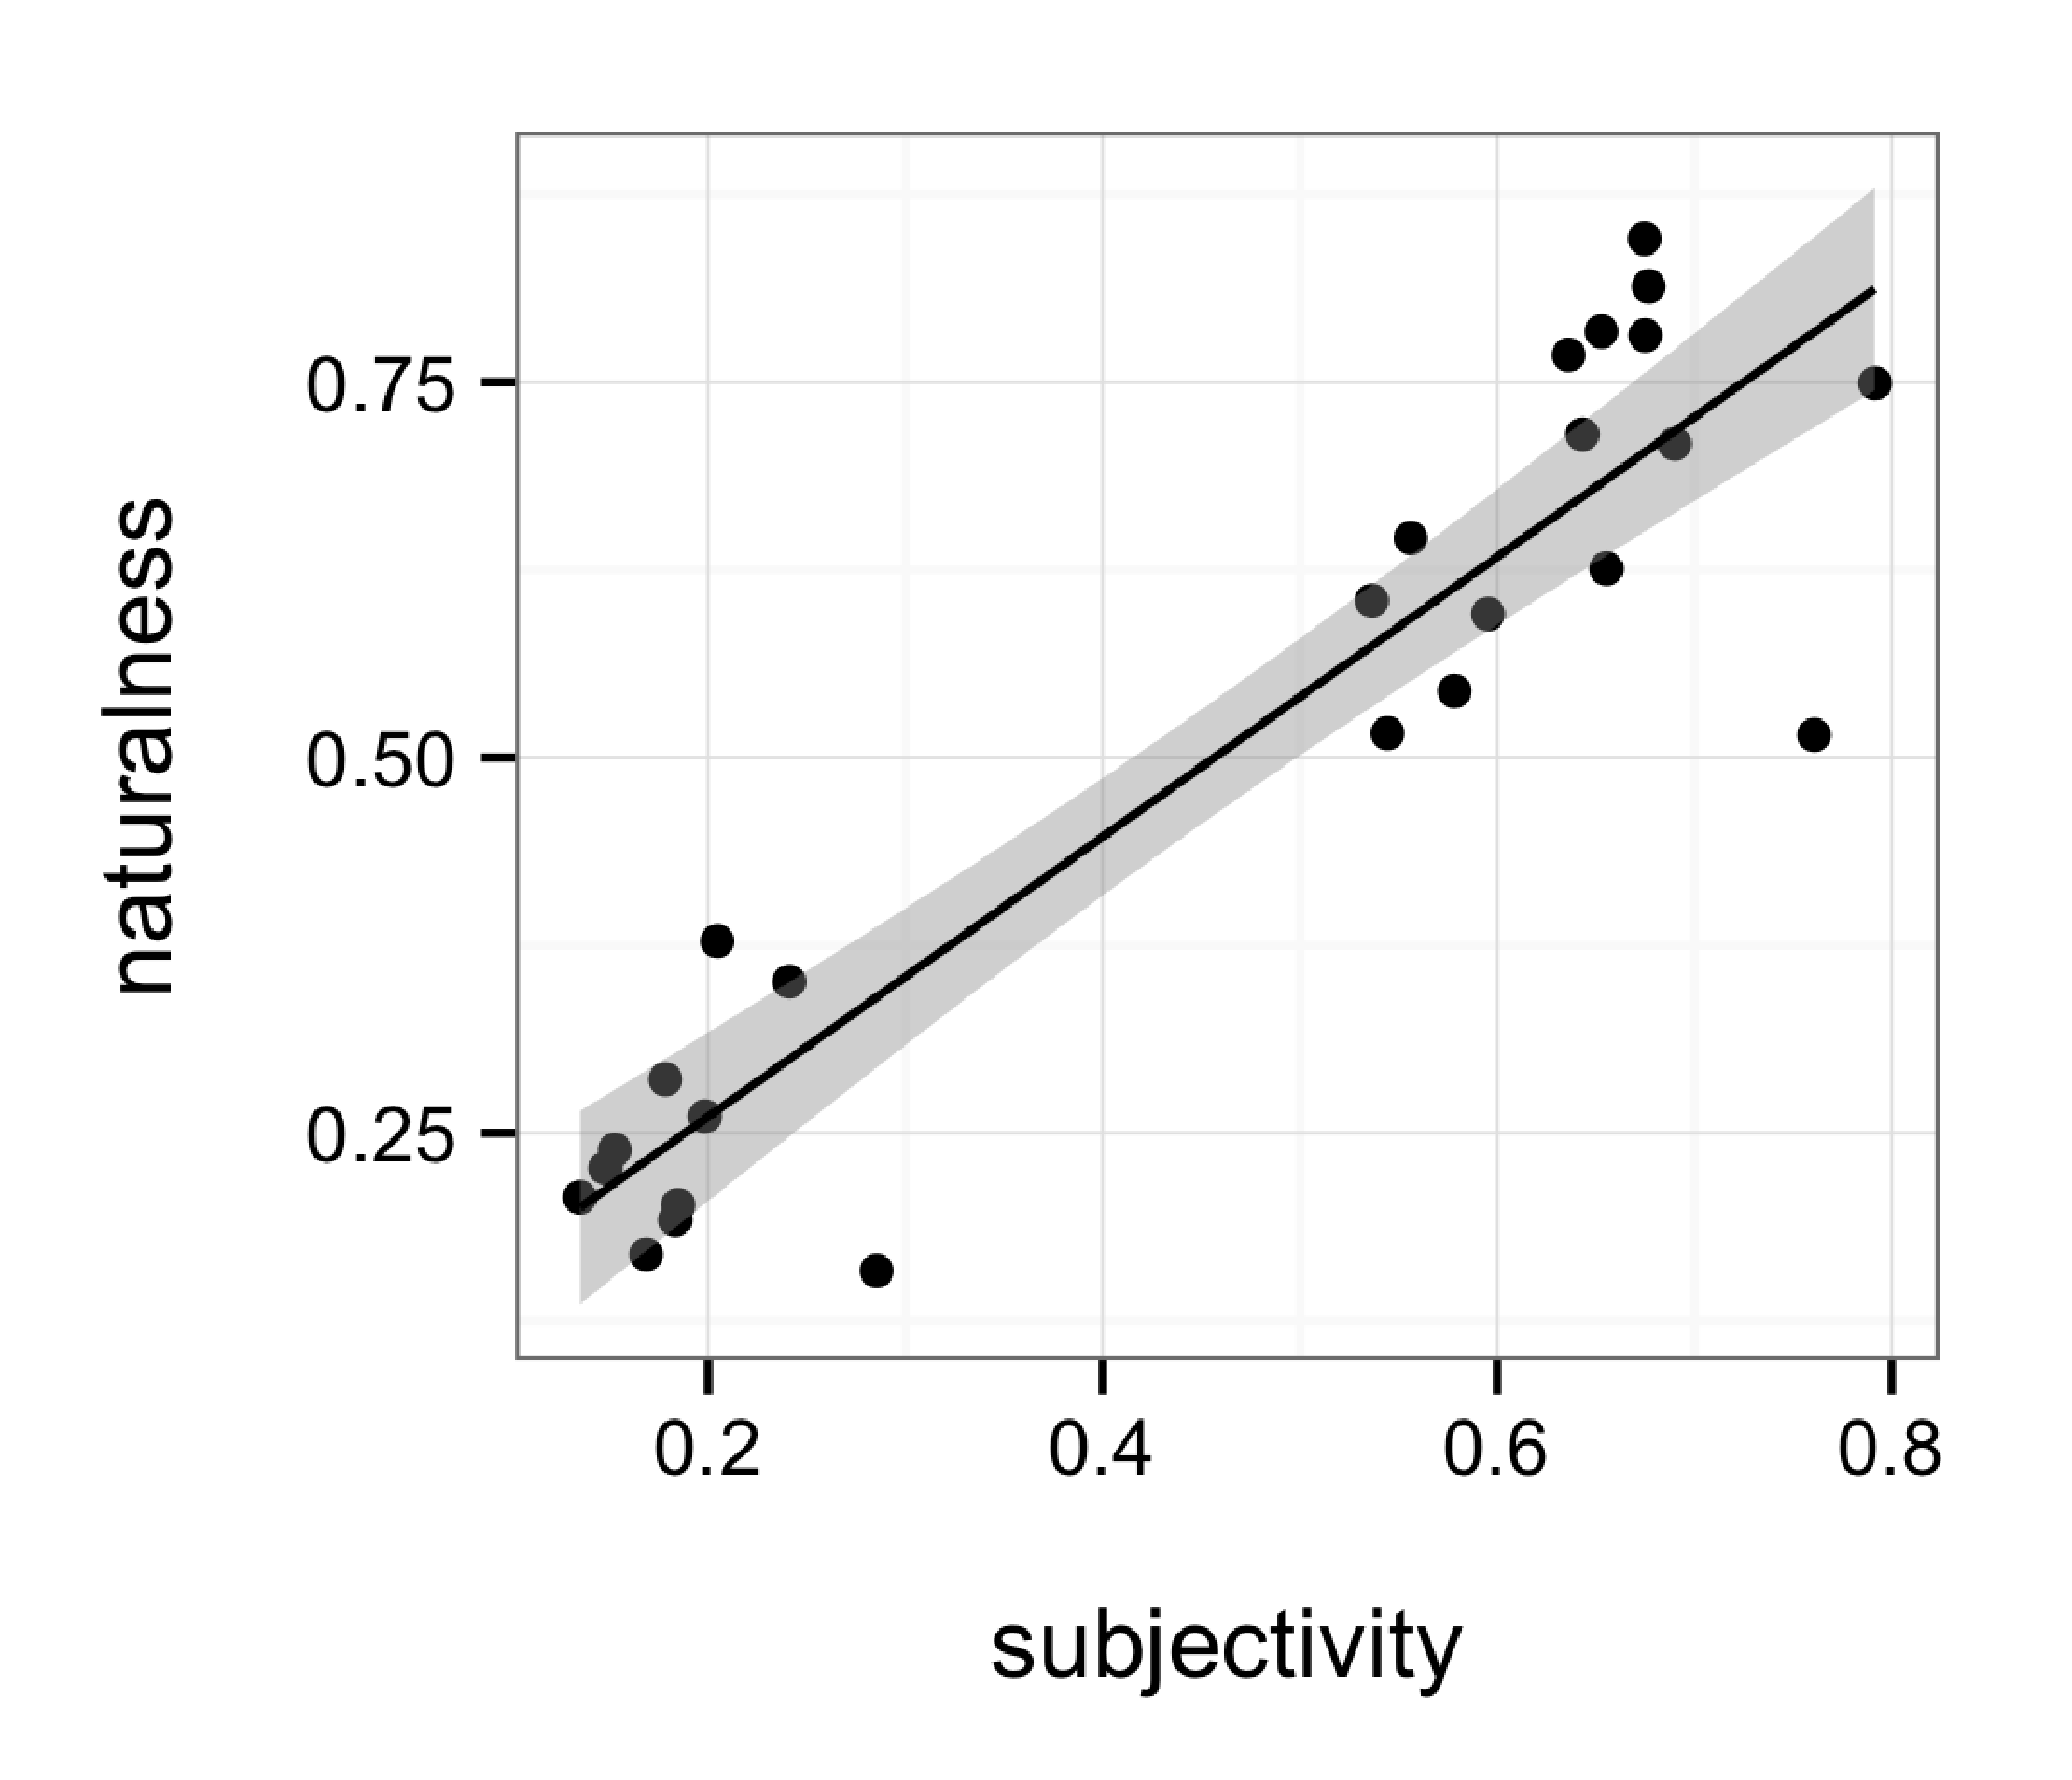
\includegraphics[width=3.5in]{plots/naturalness-subjectivity-new-nouns.eps}
	\caption{Mean naturalness ratings plotted against mean subjectivity scores for each of the 26 adjectives tested in Expt.~2.}\label{fig:subjectivity}
\end{figure}

\subsection{Discussion}

We  failed to find evidence in support of compositional accounts of ordering preferences, which hold that the most important factor in determining order is whether or not an adjective forms a complex concept with the noun it modifies. Using nouns chosen to maximize the probability of complex concepts formed with our 26 adjectives, we failed to find evidence that adjective ordering preferences depend on the modified noun. We do continue to find that subjectivity predicts ordering preferences.
It is quite possible that noun-effects (and hence effects of concept composition) would be found with a different set of adjectives. 
However, this already suggests that the effect of modified nouns explains only a small part of the overall story of adjective order; subjectivity seems to do better.

\section{Experiment 3: Generalizing our findings}

One might worry that the observed success of subjectivity in predicting ordering preferences is an artifact of the set of 26 adjectives we have so-far tested, and might not generalize to larger sets of materials. Therefore, to investigate the generalizability of our findings, in our final experiment we consider a much larger set of materials. This larger set includes many adjectives that are traditionally overlooked in investigations of ordering preferences.

\subsection{Ordering preferences}

\paragraph{Participants.} We recruited 495 participants through Amazon.com's Mechanical Turk. Participants were compensated for their participation.

\paragraph{Design and methods.}

The design was identical to our previous naturalness rating experiments (Expts.~1.1 and 2.1): participants indicated which of two object descriptions sounded more natural, choosing between adjective-adjective-noun permutations that varied the relative order of the adjectives. Adjectives were chosen at random from the set in Table \ref{tab:large-materials}, with the constraint that adjectives from the same class were not paired together.

\begin{table}
	\centering
	\caption{Adjectives used in Expt.~3.}
	\label{tab:large-materials}	
	\centering{\footnotesize\begin{tabular}{@{\vrule height 10.5pt depth2pt  width0pt}llllll}\\
	\toprule
			Adjective	&	Class	&	Adjective	&	Class	&	Adjective	&	Class	\\ \midrule
			junior	&	age	&	professional	&	human	&	sweet	&	physical	\\
new	&	age	&	sad	&	human	&	circular	&	shape	\\
old	&	age	&	selfish	&	human	&	square	&	shape	\\
old-time	&	age	&	strict	&	human	&	fast	&	speed	\\
senior	&	age	&	closest	&	location	&	slow	&	speed	\\
young	&	age	&	internal	&	location	&	speedy	&	speed	\\
black	&	color	&	overhead	&	location	&	current	&	temporal	\\
blonde	&	color	&	corduroy	&	material	&	daily	&	temporal	\\
blue	&	color	&	crocheted	&	material	&	everyday	&	temporal	\\
green	&	color	&	gold	&	material	&	historical	&	temporal	\\
purple	&	color	&	wooden	&	material	&	best	&	value	\\
red	&	color	&	brazilian	&	nationality	&	exciting	&	value	\\
white	&	color	&	english	&	nationality	&	favorite	&	value	\\
yellow	&	color	&	european	&	nationality	&	lavish	&	value	\\
biggest	&	dimension	&	hispanic	&	nationality	&	plain	&	value	\\
large	&	dimension	&	international	&	nationality	&	pleasant	&	value	\\
long	&	dimension	&	japanese	&	nationality	&	prestigious	&	value	\\
mini	&	dimension	&	national	&	nationality	&	strange	&	value	\\
narrow	&	dimension	&	vietnamese	&	nationality	&	designated	&	X	\\
open	&	dimension	&	creamy	&	physical	&	different	&	X	\\
thick	&	dimension	&	curly	&	physical	&	individual	&	X	\\
thin	&	dimension	&	frozen	&	physical	&	last	&	X	\\
civilized	&	human	&	lacy	&	physical	&	mixed	&	X	\\
creative	&	human	&	smooth	&	physical	&	potential	&	X	\\
entrepreneurial	&	human	&	solid	&	physical	&	token	&	X	\\
playful	&	human	&	spicy	&	physical	&	unique	&	X	\\	\bottomrule												
		\end{tabular}} 
\end{table}

We arrived at the new set of adjectives by extracting every unique adjective appearing in an ``A A N" NP from the Penn Treebank subset of the Switchboard corpus; there were 350 unique adjectives. Then, two of the authors (GS and JD) independently coded these 350 adjectives according to semantic classes from the literature \citep[e.g.,][]{dixon1982,Sproat1991}. We added a miscellaneous category ``X'' containing non-intersective adjectives (cf.~\citealp{Cinque2014}). After ignoring adjectives for which there was no obvious semantic class, as well as adjectives on which our classifications did not agree, we were left with 196 unique adjectives from 13 different classes.

To further refine this list of 196, we calculated adjective frequency, and on the basis of frequency divided the adjectives within each class into four quartiles. We also calculated adjective length on the basis of number of characters, and classified adjectives as either short or long. Then, for each adjective class with more than eight members, for each frequency quartile, we sampled a random adjective from each length (e.g., one short extremely frequent dimension adjective and one long extremely frequent dimension adjective). There were three cases without any observations from which to sample: ``nationality'' (Q3 short and Q4 short) and ``physical'' (Q4 short). We filled in these cases by randomly sampling from the leftovers in those two classes. Finally, we added an additional shape adjective, ``square'', because previously there was only ``circular''. This process yielded the 78 unique adjectives in Table \ref{tab:large-materials}.%, with a minimum of two adjectives from each class and a maximum of eight.

Nouns were chosen in a similar fashion. From the set of ``A A N" NPs in Switchboard, we extracted the 295 unique nouns, then restricted this set by 1) removing all plural or clearly collective nouns, and 2) removing nonsense words or words that might be confused with participles. This process yielded the 166 unique nouns in Table \ref{tab:large-materials}.

Participants completed 30 trials. On each trial, participants indicated their choice by adjusting the slider between endpoints labeled with the competing descriptions. Additionally, participants were able to indicate if a particular description did not make sense by checking a box labeled ``Neither option makes sense.'' Only native speakers of English with IP addresses located within the United States were included in the analyses; we analyzed data from 473 participants.

\paragraph{Results.}

%\begin{figure}
%	\centering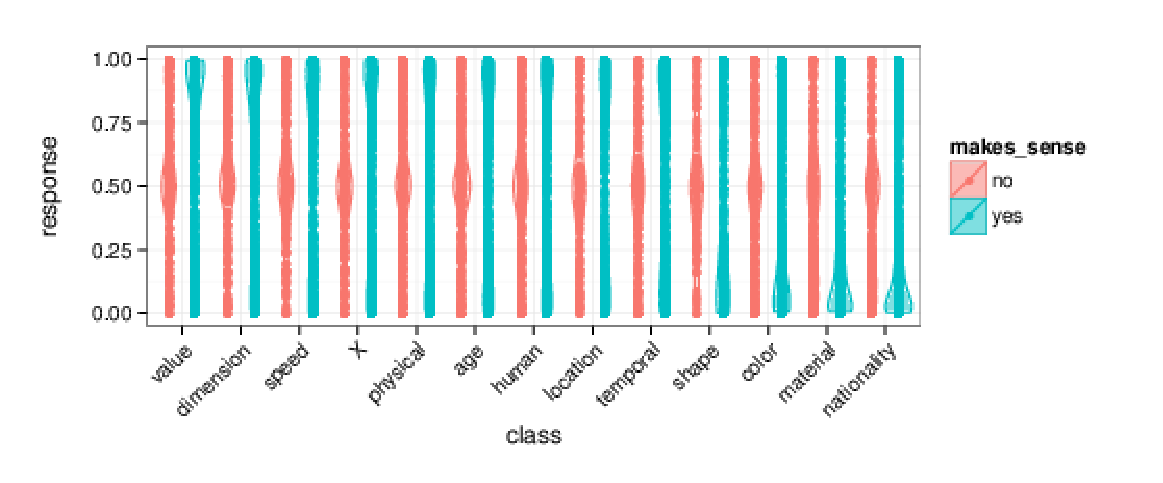
\includegraphics[width=6in]{plots/class_distance_violin.eps}
%	\caption{Mean naturalness ratings grouped by adjective class and whether or not the descriptions made sense to participants.}\label{fig:exp3-order}
%\end{figure}

Participants demonstrated little preference for adjective order when the descriptions were nonsense. For this reason, we excluded responses to nonsensical descriptions from the analyses of subjectivity below. Fig.~\ref{fig:exp3-results} (\emph{preference}) plots mean naturalness scores by adjective class for the descriptions that made sense to participants. Greater values signal that a class's adjectives are preferred in first position, farther from the modified noun; values around 0.5 indicate that neither order is preferred. 

As with the previous ordering preference experiments, we performed a nested model comparison to investigate the role of specific noun information in determining ordering preferences. The models predicted naturalness ratings either by \textsc{adjective} only, or by \textsc{adjective} together with its interaction with \textsc{noun}. Once again, the model comparison revealed that noun-specific ratings did not explain any additional variance in ordering preference above and beyond adjective-level ratings ($F(1,10100) = 0.98, p < 0.87$).

\subsection{Subjectivity}

Next, we evaluated the subjectivity of our new set of adjectives using the direct ``subjectivity'' task from Expt.~1.2.

\paragraph{Participants.}

We recruited 198 participants from Amazon.com's Mechanical Turk. Participants were compensated for their participants.

\paragraph{Design and methods.}

The design was identical to our previous direct ``subjectivity'' experiment: participants rated the subjectivity of an adjective on a sliding scale with endpoints labeled ``completely objective'' (coded as 0) and ``completely subjective'' (coded as 1). Adjectives were chosen at random from the set of 78 in Table \ref{tab:large-materials}. Participants completed a total of 30 trials. Only native speakers of English with IP addresses located within the United States were included in the analyses; we analyzed data from 189 participants.

\paragraph{Results.}

\begin{figure}
	\centering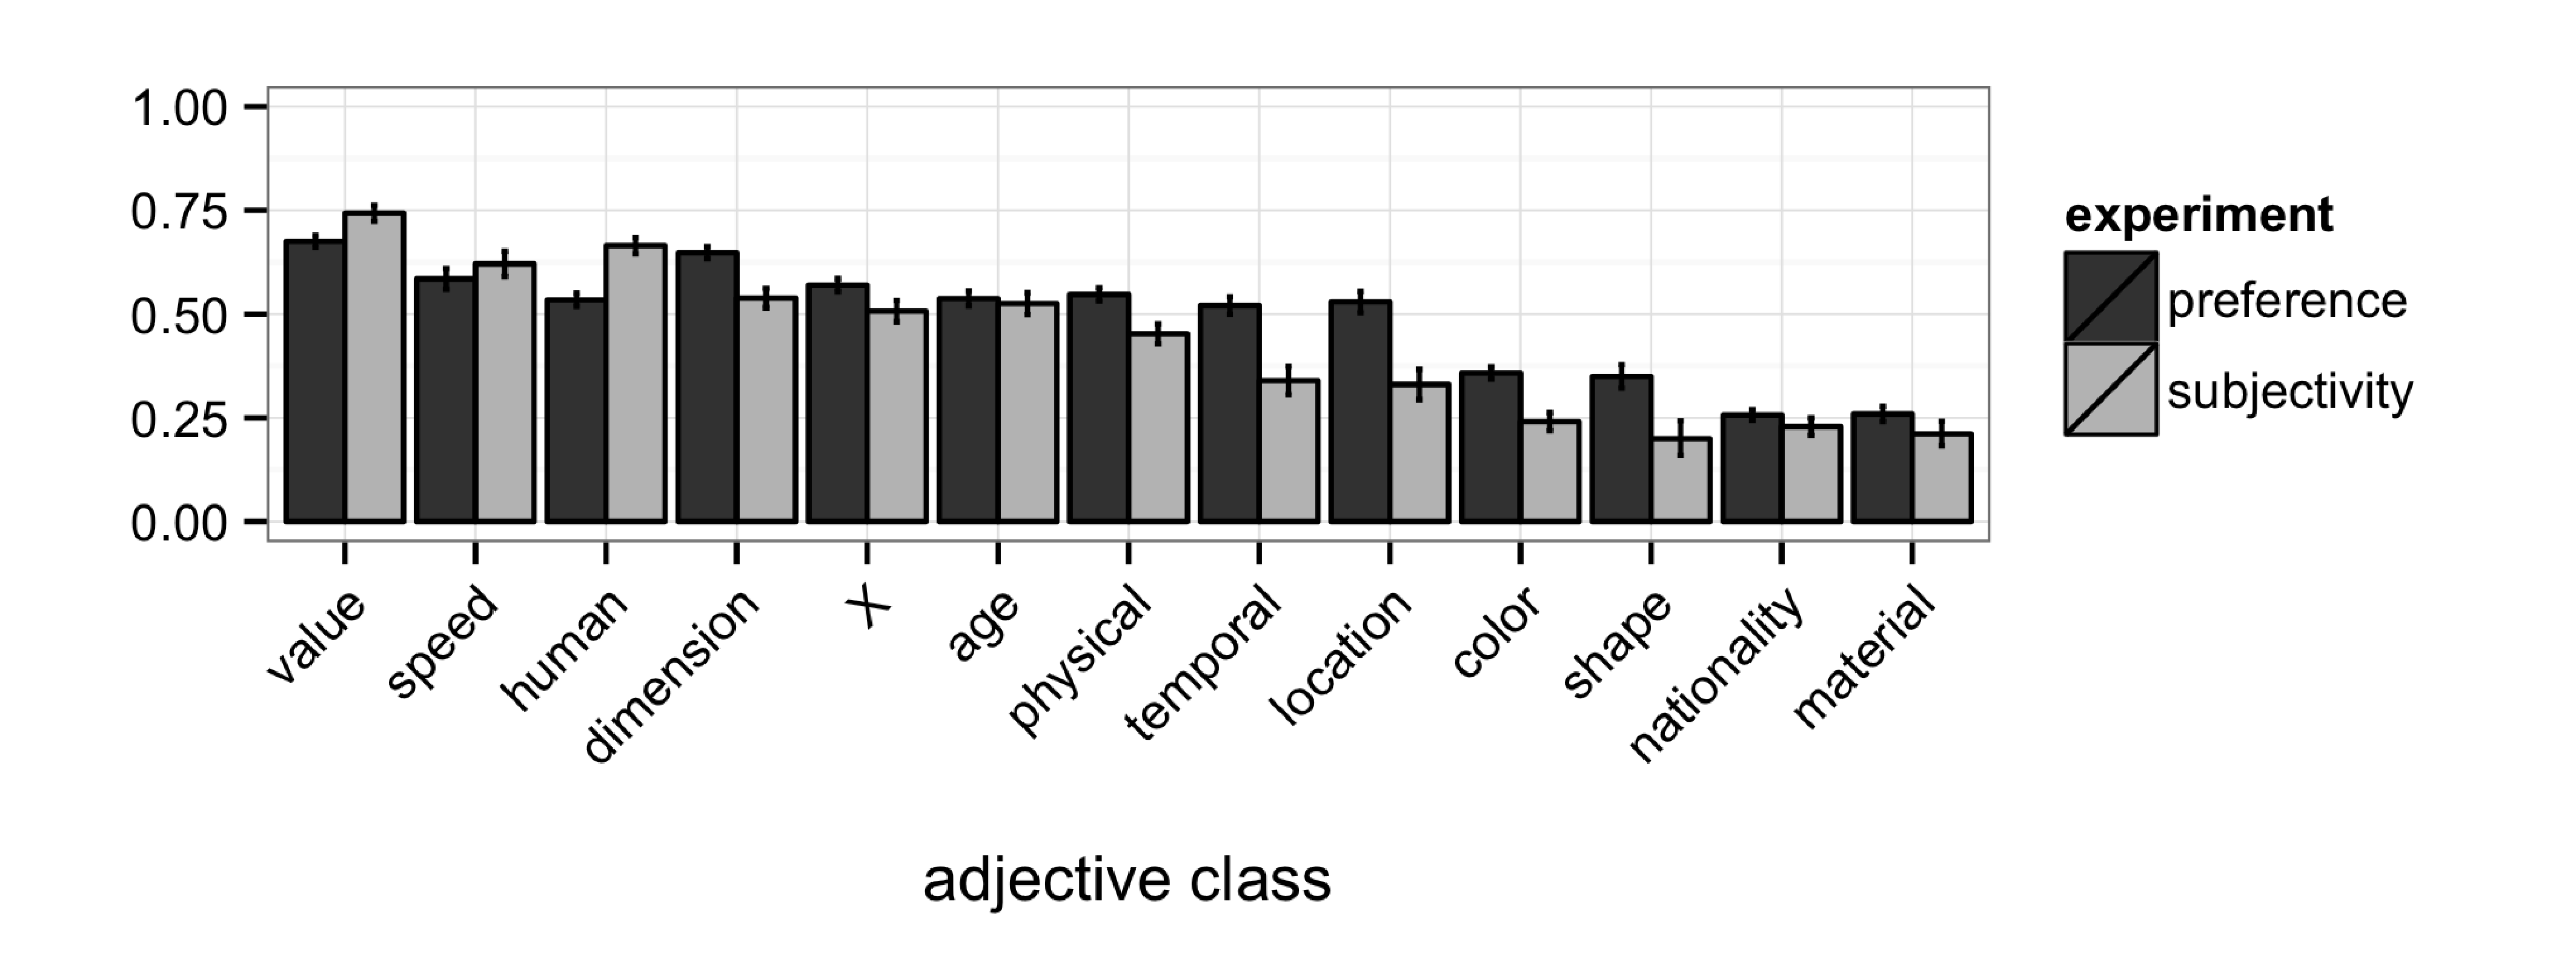
\includegraphics[width=6in]{plots/expt3_results.eps}
	\caption{Mean subjectivity ratings grouped by adjective class.}\label{fig:exp3-results}
\end{figure}

Fig.~\ref{fig:exp3-results} (\emph{subjectivity}) plots mean subjectivity scores by adjective class; greater values indicate that a class's adjectives are judged to be more subjective. To evaluate the power of subjectivity in predicting adjective ordering preferences, we compared subjectivity scores with the naturalness ratings (Fig.~\ref{fig:exp3-nat-subj}). Adjective subjectivity scores account for 51\% of the variance in the naturalness ratings ($r^2=0.51$, 95\% CI $[0.32, 0.66]$). Four observations clearly stood out in Fig.~\ref{fig:exp3-nat-subj}, corresponding to the superlatives \emph{best}, \emph{biggest}, \emph{closest}, and \emph{last}. Indeed, superlatives have been observed to eschew adjective ordering preferences, occurring farthest from the modified noun regardless of class or subjectivity \citep{dixon1982}; our naturalness ratings reflect this fact. Removing superlatives from the naturalness ratings, we find that subjectivity scores perform markedly better, accounting for 61\% of the variance ($r^2=0.61$, 95\% CI $[0.46, 0.71]$). At the level of adjective class configurations, subjectivity difference scores account for 74\% of the variance in the configuration ratings ($r^2=0.74$, 95\% CI $[0.66, 0.79]$; Fig.~\ref{fig:exp3-nat-subj-diff}).\footnote{This analysis and the plot in Fig.~\ref{fig:exp3-nat-subj-diff} exclude superlatives. If we include superlatives in the class configuration analysis, subjectivity difference scores account for 69\% of the variance in the naturalness ratings ($r^2=0.69$, 95\% CI $[0.60,  0.76]$).}

\begin{figure}
	\centering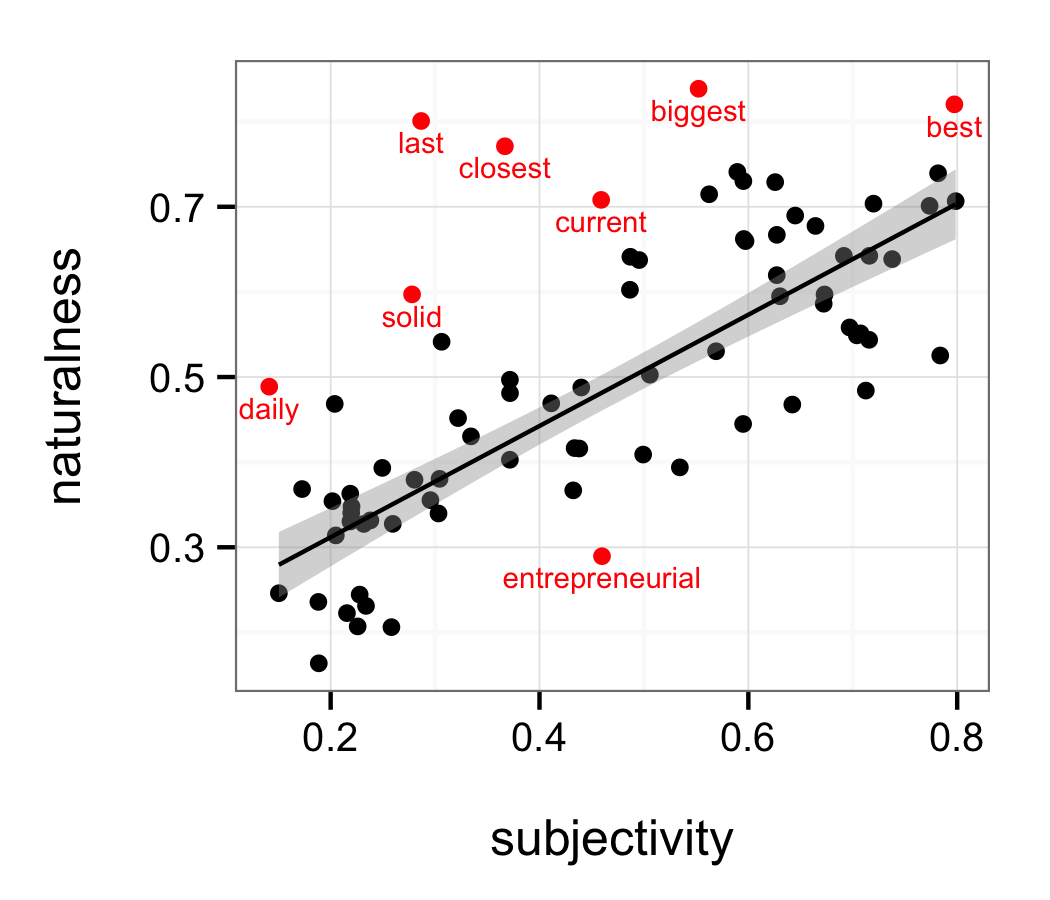
\includegraphics[width=3.5in]{plots/expt3_nat-sub.eps}
	\caption{Mean naturalness ratings plotted against mean subjectivity scores for each of the 78 adjectives tested in Expt.~3. Superlatives and outlier adjectives are labeled in red.}\label{fig:exp3-nat-subj}
\end{figure}

\begin{figure}
	\centering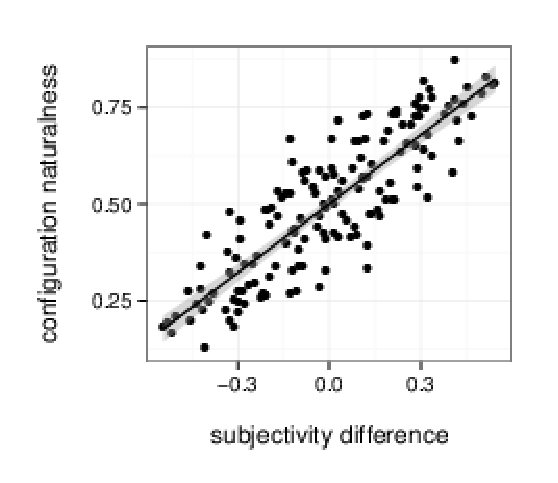
\includegraphics[width=3.5in]{plots/naturalness-subjectivity_class-difference_no-sup.eps}
	\caption{Mean configuration naturalness ratings plotted against subjectivity difference scores for each pair of adjective classes tested in Expt.~3.}\label{fig:exp3-nat-subj-diff}
\end{figure}

A post-hoc look at our data revealed a small number of outlier adjectives in addition to the four superlatives. To systematically detect these outlier adjectives, we fit a linear regression predicting naturalness ratings by subjectivity scores, then calculated the absolute difference between the actual naturalness ratings and the model's predicted values. Setting the cutoff for this difference score at 3 $\times$ standard deviation, four adjectives stood apart as outliers: ​\emph{entrepreneurial}​, ​\emph{solid}​, ​\emph{current}​, and ​\emph{daily} (labelled in red in Fig.~\ref{fig:exp3-nat-subj}). Without the four outlier adjectives (and the four superlatives), adjective subjectivity scores account for 70\% of the variance in the naturalness ratings ($r^2=0.70$, 95\% CI $[0.58,  0.78]$).

We also looked at the contribution of frequency and length in predicting ordering preferences. Treating subjectivity, frequency, and length as predictors in a linear regression predicting naturalness ratings (excluding superlatives), the model accounts for 70\% of the variance ($r^{2}=0.70$). If we remove outlier adjectives that fall more than three standard deviations away from the predicted value of the model (there were six: \emph{mini}, \emph{frozen}, \emph{solid}, \emph{current}, \emph{daily}, \emph{designated}), the model performs better, accounting for 76\% of the variance ($r^{2}=0.76)$.

\subsection{Discussion}

The results of the current experiment demonstrate that subjectivity predicts ordering preferences not just for our original set of 26 adjectives, but in a much larger set of materials drawn from naturally-occurring examples. At worst, subjectivity accounts for more than half of the variance in the naturalness ratings for our set of 78 adjectives. Once we exclude superlatives, whose semantics likely dictates their position in strings of nominal modifiers, as well as four outlier adjectives, subjectivity accounts for 70\% of the variance in this set of 70 adjectives. While adjective frequency and length contribute to the observed preferences, we saw that subjectivity alone accounts for the vast majority of the variance in our data.

There remains the question of precisely \emph{why} the four outlier adjectives---​\emph{entrepreneurial}​, ​\emph{solid}​, ​\emph{current}​, and ​\emph{daily}---performed so poorly with respect to the predictions of subjectivity. Perhaps the most notable feature of this set of adjectives is its heterogeneity: we fail to find clear groupings by semantic class, relative frequency, or length. However, length likely does factor into the observed behavior of \emph{entrepreneurial}, the longest adjective tested, which was the only outlier \emph{under}-predicted by its subjectivity: participants preferred \emph{entrepreneurial} closer to the noun than its subjectivity alone would predict. Indeed, relative length has long been known to affect the order of constituents, even in the domain of adjective ordering \citep{wulff2003}: longer constituents appear later. Once we factor length into the equation predicting ordering preferences, \emph{entrepreneurial} no longer stands out.

%With \emph{solid}, polysemy of meaning potentially contributes to its outlier status. Modifying concrete, inanimate objects, \emph{solid} receives  Finally, for the temporal adjectives \emph{current} and \emph{daily}, 

\section{General discussion}

Adjective ordering preferences have received considerable attention throughout the history of generative grammar and cognitive psychology, owing to their remarkable stability within and across languages. Something so robust, the reasoning goes, must evidence a deep principle of the cognitive architecture that shapes language. Yet while descriptions of the phenomenon abound, an explanation has proven elusive. Grammatical theories that posit a rigid syntax of adjective classes offer little more than a codification of the facts, and psychological approaches stumble when it comes to operationalizing the specific aspects of adjective meaning at play. 

In our investigation, we established two empirical constructs: the preferences themselves, which we measured using naturalness ratings and validated with corpus statistics; and adjective subjectivity, which we measured directly and corroborated with potential for faultless disagreement. 
An adjective's semantics predicts its distance from the modified noun, such that less subjective adjectives occur linearly closer to nouns they modify. 
This preference is not deterministic; non-preferred orderings of adjectives can serve a communicative purpose, for example to establish contrastiveness in discourse \citep{martin1969,Martin1970,Hill1958,vendler1963}. This constrastiveness follows straightforwardly from a manner implicature \citep{levinson2000}: marked forms (i.e., non-preferred orderings of adjectives) yield marked interpretations (i.e., atypical modification constituency). The work lies in determining the preferred orderings from which  contrastive uses depart. Indeed, many other situational factors are likely to influence ordering (e.g., phonological shape, noun semantics, word and bi-gram frequencies; cf.~\citealp{wulff2003}); it is the more general tendencies we are concerned with here.

Adjectives are just one of many elements that may occur in complex nominal constructions. Other classes of elements include demonstratives (e.g., \emph{this} and \emph{that}) and numerals. In his Universal 20, Greenberg observes that the relative order of these higher-order classes is also stable cross-linguistically \citep{greenberg1963,Culbertson2014}, suggesting that subjectivity interacts with additional constraints from semantic composition in the determination of word order. Indeed, we saw hints of such interactions in Expt.~3, where superlatives stood apart from run-of-the-mill adjectives. Beyond nominals, adverbs (e.g., \emph{honestly}, \emph{probably}, \emph{carefully}) are reported to exhibit regular orderings cross-linguistically \citep{cinque1999,ernst2002}. Understanding these orderings would likely benefit from a systematic empirical treatment similar to the one we have advanced here.

Our results suggest that ordering preferences likely emerge, at least partially, from a desire to place less subjective content closer to the substantive head of a nominal construction (i.e., closer to the modified noun). 
For now we can only speculate about the ultimate source of this desire: Subjective content allows for miscommunication to arise if speakers and listeners arrive at different judgments about a property description. Hence, less subjective content is more useful at communicating about the world. 
An explanation along these lines, based on pressures to facilitate successful reference resolution, would have to depend on the hierarchical, not linear, ordering of adjectives (cf.~the mirroring of preferences in pre- vs.~post-nominal languages). 
Whatever its source, the success of subjectivity in predicting adjective ordering preferences provides a compelling case where linguistic universals, the regularities we observe in adjective ordering, emerge from cognitive universals, the subjectivity of the properties that the adjectives name.


  \bibliographystyle{chicago} 
  \bibliography{adjectives}


\end{document}














